% Tento soubor nahraďte vlastním souborem s přílohami (nadpisy níže jsou pouze pro příklad)
% This file should be replaced with your file with an appendices (headings below are examples only)

% Umístění obsahu paměťového média do příloh je vhodné konzultovat s vedoucím
% Placing of table of contents of the memory media here should be consulted with a supervisor
%\chapter{Obsah přiloženého paměťového média}

%\chapter{Manuál}

\chapter{Obsah přiloženého paměťového média}
Součástí diplomové práce je paměťové médium, které obsahuje:

\begin{itemize}
    \item \texttt{DIP\_DistributedRepository} -- zdrojové kódy modulů distribuovaného úložiště
    
    \item \texttt{Docker} -- běhové prostředí, skripty a~Docker obrazy technologií pro běh systému
    
    \item \texttt{PCAP\_Input} -- adresář, jehož cesta je předána klientské demo aplikaci ve spouštěcím skriptu, slouží jako zdroj PCAP souborů k~odeslání do distribuovaného úložiště
    
    \item \texttt{SEP\_DistributedRepository} -- zdrojové kódy modulů prototypu
    
    \item \texttt{Text} -- zdrojové kódy k~technické zprávě včetně všech diagramů ve formátu PDF a~formátu pro grafický online nástroj \texttt{draw.io} \footnote{https://www.draw.io/}
    
    \item \texttt{LICENSE} -- licence systému
    
    \item \texttt{README.md} -- návod k~běhovému prostředí a~ke spuštění systému
\end{itemize}

\chapter{Konfigurace} \label{configuration}
\section{Systém distribuovaného úložiště}
Konfigurace aplikace DistributedRepository se nachází v~souboru \\ \texttt{DistributedRepository/src/main/resources/application.properties} \\
a~obsahuje tyto položky:

\vspace{0.5cm}
\noindent \texttt{\#   Cassandra \\
spring.data.cassandra.keyspace-name=structured\_data \\
spring.data.cassandra.contact-points=192.168.99.100 \\
spring.data.cassandra.port=9042 \\
\#   Hadoop \\
spring.hadoop.fs-uri=hdfs://172.17.0.4:9000 \\
\#   Kafka \\
spring.kafka.bootstrap-servers=192.168.99.100:9092 \\
spring.kafka.consumer.auto-commit-interval=1000 \\
spring.kafka.consumer.enable-auto-commit=true \\
spring.kafka.consumer.group-id=test \\
spring.kafka.consumer.key-deserializer= \\
\indent cz.vutbr.fit.communication.serialization.KafkaRequestDeserializer \\
spring.kafka.consumer.value-deserializer= \\
\indent org.apache.kafka.common.serialization.ByteArrayDeserializer \\
spring.kafka.producer.acks=all \\
spring.kafka.producer.batch-size=16384 \\
spring.kafka.producer.bootstrap-servers=192.168.99.100:9092 \\
spring.kafka.producer.buffer-memory=335544320 \\
spring.kafka.producer.key-serializer= \\
\indent cz.vutbr.fit.communication.serialization.KafkaResponseSerializer \\
spring.kafka.producer.properties.max.request.size=500000000 \\
spring.kafka.producer.retries=0 \\
spring.kafka.producer.value-serializer= \\
\indent org.apache.kafka.common.serialization.ByteArraySerializer \\
input.topic=input\_topic \\
output.topic=output\_topic \\
error.topic=error\_topic \\
\#   Logging \\
logging.level.cz.vutbr.fit=DEBUG \\
logging.level.org.pcap4j.core=INFO \\
\#   MongoDB \\
spring.data.mongodb.host=192.168.99.100 \\
spring.data.mongodb.port=27017 \\
spring.data.mongodb.database=metadata \\
\#   StorePcapHandler \\
packet.metadata.max.list.size=500 \\
tmp.directory=tmp/
}

\section{Klientská aplikace}
Konfigurace aplikace ProducerDemo se nachází v~souboru \\
\texttt{ProducerDemo/src/main/resources/application.properties} \\
a~obsahuje tyto položky:

\vspace{0.5cm}
\noindent \texttt{\#   Hadoop \\
spring.hadoop.fs-uri=hdfs://172.17.0.4:9000 \\
\#   Kafka \\
spring.kafka.bootstrap-servers=192.168.99.100:9092 \\
spring.kafka.consumer.auto-commit-interval=1000 \\
spring.kafka.consumer.enable-auto-commit=true \\
spring.kafka.consumer.group-id=test \\
spring.kafka.consumer.key-deserializer= \\
\indent cz.vutbr.fit.communication.serialization.KafkaResponseDeserializer \\
spring.kafka.consumer.value-deserializer= \\
\indent org.apache.kafka.common.serialization.ByteArrayDeserializer \\
spring.kafka.producer.acks=all \\
spring.kafka.producer.batch-size=16384 \\
spring.kafka.producer.bootstrap-servers=192.168.99.100:9092 \\
spring.kafka.producer.buffer-memory=335544320 \\
spring.kafka.producer.key-serializer= \\
\indent cz.vutbr.fit.communication.serialization.KafkaRequestSerializer \\
spring.kafka.producer.properties.max.request.size=500000000 \\
spring.kafka.producer.retries=0 \\
spring.kafka.producer.value-serializer= \\
\indent org.apache.kafka.common.serialization.ByteArraySerializer \\
input.topic=input\_topic \\
output.topic=output\_topic \\
error.topic=error\_topic \\
\#   Logging \\
logging.level.cz.vutbr.fit=DEBUG \\
\#   StorePcapProducerDemo \\
cz.vutbr.fit.producerdemo.demo.StorePcapProducerDemo.dataSourceStorage=HDFS \\
\#   LoadPcapProducerDemo \\
cz.vutbr.fit.producerdemo.demo.LoadPcapProducerDemo.dataSourceStorage=HDFS
}

\chapter{Běhové prostředí} \label{dockerEnv}
Jako běhové prostředí pro systém distribuovaného repositáře byl zvolen projekt Docker \footnote{https://www.docker.com/} z~důvodu jednodušší a~oddělené správy použitých technologií. Každá technologie běží v~odděleném kontejneru spuštěném z~předem připraveného obrazu. Všechny soubory a~skripty týkající se běhového prostředí jsou uloženy v~adresáři \texttt{Docker}.

\section{Obrazy}
Každou technologii reprezentuje samostatný obraz (angl. \texttt{image}), v~němž je daná technologie nainstalována.

\vspace{0.5cm}
\noindent Kompletní přehled obrazů:

\begin{lstlisting}[language=bash,basicstyle={\small\ttfamily}]
$ docker image ls
REPOSITORY                  TAG                 IMAGE ID         CREATED          SIZE
martinfit/maven             3.5.2-jdk-9-slim    b78e23733813     3 hours ago      449MB
martinfit/cassandra         3                   9a1473c2fc55     3 hours ago      323MB
wurstmeister/kafka          1.0.1               2e0c23534746     2 weeks ago      330MB
mongo                       3.4                 9ad59b0c0624     3 weeks ago      360MB
cassandra                   3                   c6b513da2ff3     4 weeks ago      323MB
maven                       3.5.2-jdk-9-slim    58405637ffbb     8 weeks ago      392MB
wurstmeister/zookeeper      latest              351aa00d2fe9     16 months ago    478MB
sequenceiq/hadoop-docker    2.7.1               42efa33d1fa3     2 years ago      1.76GB
\end{lstlisting}

\noindent Většina výše uvedených obrazů pochází přímo z~oficiálního repositáře \texttt{Docker Hub} \footnote{https://hub.docker.com/}. Výjimku tvoří obrazy \texttt{martinfit/maven} a~\texttt{martinfit/cassandra}. Tyto dva obrazy jsou založeny na obrazech z~Docker Hub, ale byla do nich přidána dodatečná konfigurace. Obraz pro databázi Cassandra byl mírně upraven, aby bylo možné inicializovat schéma databáze při spuštění kontejneru. Do obrazu pro nástroj Maven byla doinstalována nativní knihovna \texttt{libpcap} kvůli korektnímu běhu knihovny Pcap4J \ref{pcap4j}.

Instalaci prostředí (tzn. stažení a~sestavení obrazů) provádí nástroje \texttt{docker-compose pull} a~\texttt{docker build} uvnitř skriptu \texttt{install-docker-enviroment.sh}. Spuštění kontejnerů z~definovaných obrazů zajistí skript \texttt{run-docker-enviroment.sh}. Zastavit kontejnery lze pomocí skriptu \texttt{stop-docker-enviroment.sh}. Veškerá konfigurace obrazů a~kontejnerů se nachází v~souboru \texttt{Environment/docker-compose.yml}.

\chapter{Spuštění aplikací} \label{launching}
Sestavení jednotlivých modulů zajišťují přiložené skripty \texttt{install.sh} v~adresáři každého modulu. Jednotlivé cesty ke skriptům jsou:

\begin{enumerate}
    \item \texttt{Communication/install.sh}
    
    \item \texttt{Persistence/install.sh}
    
    \item \texttt{DistributedRepository/install.sh}
    
    \item \texttt{ProducerDemo/install.sh}
\end{enumerate}

\noindent Kvůli závislostem mezi moduly je nutné skripty spustit ve výše uvedeném pořadí. Moduly jsou zkompilovány a~sestaveny pomocí nástroje Maven, který provede stažení všech potřebných závislostí.

\section{DistributedRepository}
Systém distribuovaného úložiště lze spustit skriptem \texttt{DistributedRepository/run.sh}, který dynamicky zjistí IP adresy běžících kontejnerů v~Docker, a~na základě zjištěných hodnot přepíše aplikační proměnné.

\section{ProducerDemo}
Klientskou aplikaci lze spustit pomocí skriptu \texttt{ProducerDemo/run.sh}, který také dynamicky přepíše aplikační proměnné podle běžících kontejnerů.

\chapter{Data z~měření výkonnosti}

\section{Prototyp}

\begin{table}[h!]
    \centering
    \begin{tabular}{| l | l | l | l | l |}
    \hline
    \texttt{PCAP size (B)}   &   \texttt{Count of packets}   &   \texttt{Avg. packet size} &  \texttt{Time (s)} &   \texttt{Packets/s} \\ \hline
    91 340 & 382 & 239,1099476 & 7 & 54,57142857 \\ \hline
    1 955 172 & 1360 & 1437,626471 & 13 & 104,6153846 \\ \hline
    412 254 & 1879 & 219,4007451 & 19 & 98,89473684 \\ \hline
    420 869 & 2263 & 185,9783473 & 23 & 98,39130435 \\ \hline
    449 234 & 2563 & 175,276629 & 29 & 88,37931034 \\ \hline
    \end{tabular}\par
    \bigskip
    \caption{Tabulka obsahuje data naměřená při testování výkonnosti prototypu.}
    \label{tablePerformancePrototype}
\end{table}

\section{Finální systém}

\begin{table}[h!]
    \centering
    \begin{tabular}{| l | l | l | l | l |}
    \hline
    \texttt{PCAP size (B)}   &   \texttt{Count of packets}   &   \texttt{Avg. packet size} &  \texttt{Time (s)} &   \texttt{Packets/s} \\ \hline
    91 340 & 382 & 239,1099476 & 0,5 & 764 \\ \hline
    1 955 172 & 1360 & 1437,626471 & 0,5 & 2720 \\ \hline
    412 254 & 1879 & 219,4007451 & 0,5 & 3758 \\ \hline
    420 869 & 2263 & 185,9783473 & 1 & 2263 \\ \hline
    449 234 & 2563 & 175,276629 & 1,5 & 1709 \\ \hline
    \end{tabular}\par
    \bigskip
    \caption{Tabulka obsahuje data naměřená při testování výkonnosti finálního systému.}
    \label{tablePerformanceFinalSystem}
\end{table}

\chapter{Diagram tříd prototypu}

\begin{figure}[!h]
    \centering
    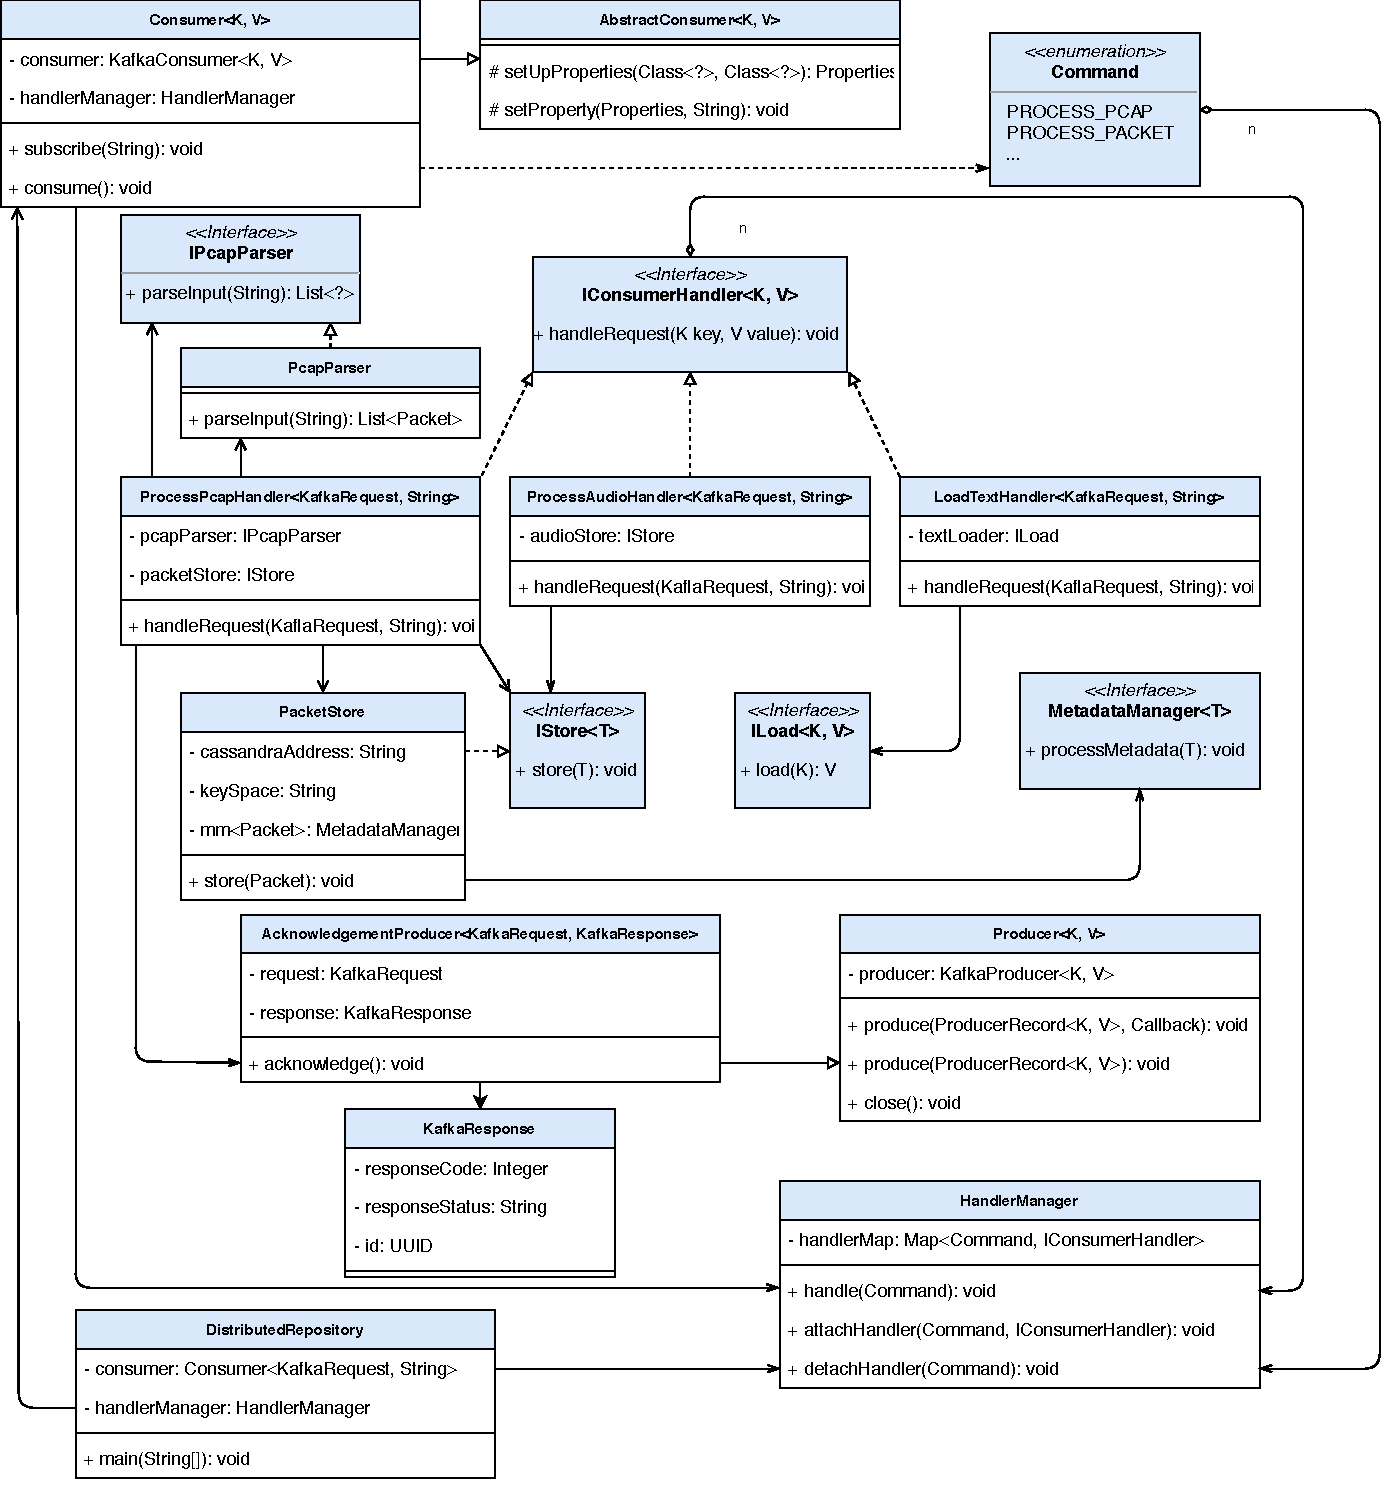
\includegraphics[width=14.35cm]{template-fig/Prototype_ClassDiagram.pdf}
    \caption{Diagram tříd prototypu.}
    \label{FIG_PrototypeClassDiagram}
\end{figure}
